% An atomic (linearizable) history involving two registers
% for demonstrating the locality property of atomicity.

\documentclass{standalone}

\usepackage{tikz}

\tikzset{wop/.style = {blue, very thick},
  rop/.style = {brown, very thick}}

% interval for operations
\newcommand{\itv}[5]{ % #1: start point; #2: end point; #3: operation name; #4: style; #name
  \coordinate (start #3) at #1;	% start point
  \coordinate (end #3) at #2;	% end point

  \draw[#4, |-|] (start #3) -- (end #3) % draw the interval
  node[pos = 0.5, above = 1mm, font = \Large] (#5) {\textsl{#3}}; % attach the operation name
}

\begin{document}
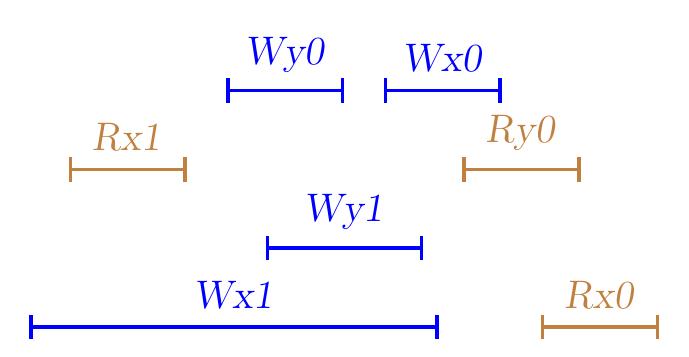
\begin{tikzpicture}
  \itv{(0,0)}{(5.2,0)}{Wx1}{wop}{wx1}
  \itv{(6.5,0)}{(8,0)}{Rx0}{rop}{rx0}

  \itv{(3,1)}{(5,1)}{Wy1}{wop}{wy1}

  \itv{(0.5,2)}{(2,2)}{Rx1}{rop}{rx1}
  \itv{(5.5,2)}{(7,2)}{Ry0}{rop}{ry0}

  \itv{(2.5,3)}{(4,3)}{Wy0}{wop}{wy0}
  \itv{(4.5,3)}{(6,3)}{Wx0}{wop}{wx0}
\end{tikzpicture}
\end{document}
